\documentclass[conference]{IEEEtran}

\usepackage[T1]{fontenc}
\usepackage[utf8]{inputenc}
\usepackage{amsmath,amssymb}
\usepackage{graphicx}
\usepackage[caption=false,font=footnotesize]{subfig}
\usepackage{flushend}
\usepackage{microtype}
\usepackage[colorlinks=true,linkcolor=blue,citecolor=blue,urlcolor=blue]{hyperref}

\begin{document}

\title{Placing \texorpdfstring{$K$}{K} Disks of Radius \texorpdfstring{$R$}{R} to Cover the Most Households}

\author{
\IEEEauthorblockN{Kri\v{s}j\={a}nis Petru\v{c}e\c{n}a}
\IEEEauthorblockA{University of Latvia}
}

\maketitle

\begin{abstract}
We study the placement of $K$ disks of radius $R$ so as to cover as many as possible of $N$ given points in the plane.
The points are households with integer coordinates.
Each disk is a cellular tower with range $R$.
The continuous placement problem has an equivalent discrete candidate set of size $O(N^2)$.
This note records a clustered benchmark on the integer square $[0,100]\times[0,100]$ with $R=10$, and the solver: multi-start naive hill-climbing as the baseline, then tabu search.
\end{abstract}

\begin{IEEEkeywords}
disk coverage, facility location, local search, synthetic spatial data
\end{IEEEkeywords}

\section{Introduction}

A cellular operator may install only $K$ towers.
Each tower covers every household within distance $R$.
The operator wants to cover as many households as possible.

That story is the maximum-coverage problem with $K$ equal disks of radius $R$.
The input is $N$ points with integer coordinates, a budget $K\in\mathbb{N}$, and a radius $R>0$.
A feasible solution is $K$ centres in $\mathbb{R}^2$.
A point $p$ is covered if some centre $c$ satisfies $\|p-c\|_2\le R$.
The objective is the number of covered points.
Code and instances are at \url{https://github.com/KrisjanisP/disk-coverage-optimization-homework}.

Deciding whether $K$ equal disks can cover a given point set is NP-complete~\cite{Megiddo1984}.
Covering \emph{every} point with as few equal disks as possible admits a polynomial-time approximation scheme (PTAS) via the shifting strategy~\cite{Hochbaum1985}.
The budgeted variant is at least as hard: the yes-instances are those for which the maximum coverage equals $N$.

An optimal centre can always be moved until the disk is a smallest enclosing disk of the covered set, determined by one, two, or three points on the boundary.
Keeping those disks of radius at most $R$ yields $O(N^3)$ candidates.
A strictly smaller equivalent set has size $O(N^2)$: for every pair at distance at most $2R$ there are at most two disks of radius $R$ through both points, together with the input points themselves.
On a map with thousands of locations that set is too large to scan as a neighbourhood, so we snap each centre onto the integer lattice (displacement at most $1/\sqrt{2}$).
With $R=10$ the snap is a tenth of the covering radius.
Coverage is still Euclidean distance $\le R$.
The search chooses $K$ snapped candidates.

\section{Benchmark instance}

Households concentrate in cities.
Place $C=8$ impulses of unequal weight on a $512\times 512$ grid, convolve with a Gaussian of $\sigma=20$ pixels, and mix in a uniform floor of $12\%$ of the density mass.
Sample $N=10\,000$ locations with replacement, add unit-square jitter, scale onto a square of side $100$, and round to $\{0,\ldots,100\}$.
Fig.~\ref{fig:houses} shows those integer houses.
A city blob is about $10$ units across, matching $R=10$, so a single disk covers most of a city.
The hinterland houses are the ones the extra towers compete for.
The instance stores $K=12$ and $R=10$.
Rounding leaves $3148$ distinct cells.

\begin{figure*}[!t]
\centering
\begin{tabular}{@{}c@{\hspace{1.2em}}c@{}}
\subfloat[Integer houses on the side-$100$ map.]{%
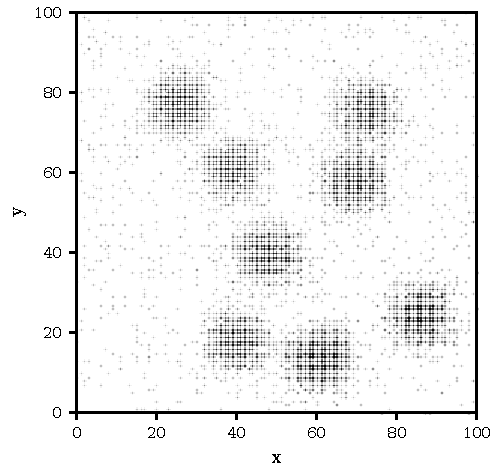
\includegraphics[width=0.38\textwidth]{figures/sampled-houses.pdf}%
\label{fig:houses}}
&
\subfloat[Tabu placement after $120$\,s ($9117$ covered).]{%
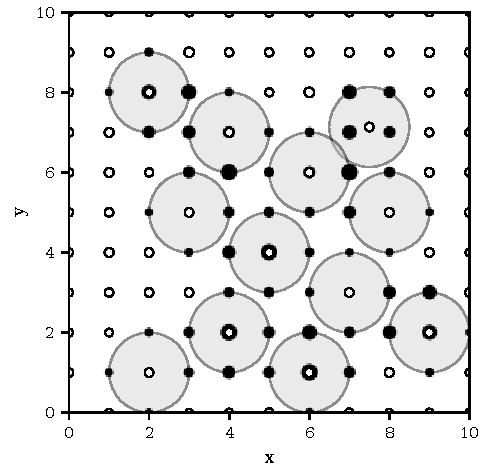
\includegraphics[width=0.38\textwidth]{figures/placement-tabu.pdf}%
\label{fig:placement}}
\\[0.6em]
\subfloat[Same disks on all $10\,000$ houses.]{%
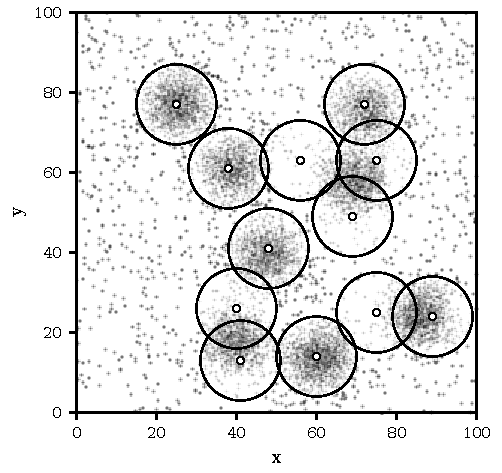
\includegraphics[width=0.38\textwidth]{figures/placement-tabu-houses.pdf}%
\label{fig:placement-houses}}
&
\subfloat[Best-so-far uncovered count ($896$ vs $883$).]{%
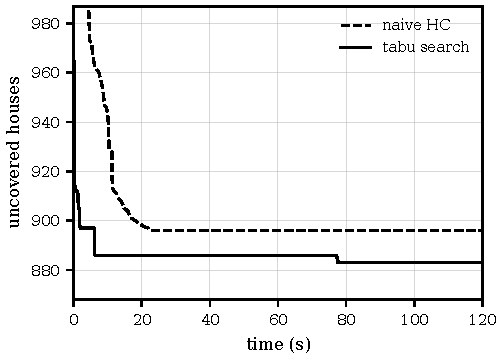
\includegraphics[width=0.38\textwidth]{figures/cost-best.pdf}%
\label{fig:cost-best}}
\end{tabular}
\caption{Houses, submitted tabu disks of radius $R=10$, and the $120$\,s comparison.
In (b), filled markers are covered cells (area $\propto$ household count) and open markers are uncovered.}
\label{fig:results}
\end{figure*}

\section{Method}

The assignment requires one self-written local-search algorithm, not a solver library.
Late-acceptance hill-climbing~\cite{Burke2017} did not beat multi-start hill-climbing on this neighbourhood, so we switch to tabu search~\cite{Glover1989}.
The baseline is naive first-improvement hill-climbing until a full neighbourhood pass finds no improving move, then a new random $K$-subset, for a two-minute budget.
Tabu search gets the same wall-clock.

\subsection{Domain}

A solution is a list of $K$ candidate centres, without repetition.
The candidate set is the snapped $O(N^2)$ radius-$R$ centres of Section~I.

\subsection{Evaluation}

Cost is the number of uncovered houses, $N$ minus the number of points within distance $R$ of at least one chosen centre.
Lower is better, matching the lecture's acceptance tests.

\subsection{Move}

A neighbour replaces one chosen centre with a different candidate: a $1$-swap in the snapped candidate set.

\subsection{Algorithm}

Tabu search starts from a random $K$-subset.
It first climbs with first-improvement: slots in random order, and on the first slot that has a better centre, the best unused candidate for that slot is taken.
A sparse candidate-by-house matrix makes that scan cheap (about $7$\,ms for all $11822$ centres).
From the local minimum, each further step takes the lowest-cost admissible $1$-swap over the whole neighbourhood.
The centre just evicted may not return for a tenure of $12$ steps, unless the swap beats the global best (aspiration).
If the global best is unchanged for $80$ tabu steps, we restart from a new random $K$-subset.
Naive hill-climbing is the same neighbourhood with no memory and with random restarts until the time budget expires.

\section{A timed comparison}

Both methods received $120$\,s on the $N=10\,000$, $K=12$, $R=10$ map ($3148$ distinct cells, $11822$ snapped candidates).
Naive multi-start hill-climbing covered $9104$ houses after $6$ local minima.
Tabu search covered $9117$ houses after $197$ restarts ($3715$ climbing steps and $16016$ tabu steps).
Evaluating each swap in Python took about $4$\,s per full scan; with the sparse matrix, tabu sees the whole $1$-swap list and still restarts far more often than the naive climber.
An integer program on the $11822$ candidates did not return a feasible incumbent within $60$\,s, so $9117$ is the best-known value on this run.
Fig.~\ref{fig:results} shows the houses, the tabu disks, and the best-so-far cost traces.
Late-acceptance hill-climbing is not the submitted method.

\bibliographystyle{IEEEtran}
\bibliography{refs}

\end{document}
